\documentclass[11pt,a4paper]{article}

\usepackage[margin=1in]{geometry}
\usepackage{amsmath,amssymb}
\usepackage{booktabs}
\usepackage{graphicx}
\usepackage{hyperref}
\usepackage{siunitx}
\usepackage{float}
\usepackage{enumitem}

\hypersetup{colorlinks=true, linkcolor=blue, urlcolor=blue, citecolor=blue}

\title{Technical Report Update: UWB--IMU Fusion Result on 260429 Dataset}
\author{Package: \texttt{uwb\_imu\_fusion}}
\date{Input CSV: \texttt{output/uwb\_imu\_trajectory\_tc\_260429.csv}}

\begin{document}
\maketitle

\begin{abstract}
This report updates the analysis of the tightly coupled UWB--IMU pipeline launched by \texttt{uwb\_imu\_fusion.launch}. The analyzed CSV contains 4,075 UWB cycles over \SI{112.73}{s}. The new result keeps the same estimator structure: a UWB-only Gauss--Newton WLS front end and a tightly coupled GTSAM/iSAM2 back end with raw TDOA factors, IMU preintegration, bias evolution, WLS priors, vertical stabilization, attitude stabilization, and WLS rescue anchoring. The main result is that WLS remains better in overall 3D RMSE, while TC improves vertical accuracy and provides a smoother full navigation state.
\end{abstract}

\section{Pipeline Summary}

The active baseline is \texttt{launch/uwb\_imu\_fusion.launch}. The node subscribes to IMU, UWB TDOA, and ground-truth pose topics. Each UWB cycle is processed in two parallel branches:

\begin{enumerate}[leftmargin=*]
  \item \textbf{WLS front end:} solves a UWB-only nonlinear least-squares position estimate from TDOA measurements.
  \item \textbf{TC-FGO back end:} inserts raw TDOA factors and one preintegrated IMU factor into an incremental GTSAM graph.
\end{enumerate}

The corrected baseline also constrains the failure mode observed in the previous report:

\begin{itemize}[leftmargin=*]
  \item roll/pitch are softly constrained near the leveled startup attitude;
  \item yaw is left effectively free;
  \item if WLS and TC separate by more than \SI{0.25}{m} in XY, a stronger WLS rescue prior is activated.
\end{itemize}

\section{Measurement Models}

For anchors \(a_A\) and \(a_B\), the WLS residual is
\begin{equation}
  r_i(p) = \left(\|p-a_B\|-\|p-a_A\|\right)-z_i ,
\end{equation}
with Jacobian
\begin{equation}
  \frac{\partial r_i}{\partial p}
  =
  \frac{p-a_B}{\|p-a_B\|}
  -
  \frac{p-a_A}{\|p-a_A\|}.
\end{equation}

The graph state at UWB cycle \(k\) is
\begin{equation}
  \mathcal{X}_k = \{X_k, v_k, b_k\},
\end{equation}
where \(X_k\in SE(3)\), \(v_k\in\mathbb{R}^3\), and \(b_k\) is the IMU bias. The TC graph minimizes the combined factor objective
\begin{equation}
  \min_{\mathcal{X}_{0:k}}
  \sum_i \|e^{\mathrm{tdoa}}_{k,i}\|_{\Sigma_{\mathrm{tdoa}}}^2
  + \|e^{\mathrm{imu}}_k\|_{\Sigma_{\mathrm{imu}}}^2
  + \|b_k-b_{k-1}\|_{\Sigma_b}^2
  + \|v_k-\hat{v}_k\|_{\Sigma_v}^2
  + \|X_k-\hat{X}^{\mathrm{wls}}_k\|_{\Sigma_{\mathrm{wls}}}^2
  + \|X_k-\hat{X}^{\mathrm{att}}\|_{\Sigma_{\mathrm{att}}}^2 .
\end{equation}
The last term is the new roll/pitch stabilization prior. Its translation components and yaw are left loose, while roll/pitch are constrained with the launch default \(\sigma=0.05\) rad.

\section{Accuracy Result}

\begin{table}[H]
  \centering
  \caption{3D position error statistics in meters for the 260429 CSV.}
  \begin{tabular}{lrrrrrr}
\toprule
Estimator & Mean & Median & RMSE & 75\% & 95\% & Max \\
\midrule
WLS UWB-only & 0.184 & 0.141 & 0.217 & 0.264 & 0.400 & 0.570 \\
TC UWB+IMU & 0.197 & 0.143 & 0.235 & 0.292 & 0.438 & 0.621 \\
\bottomrule
\end{tabular}

  \label{tab:metrics260429}
\end{table}

The WLS-only branch gives mean error \SI{0.184}{m} and RMSE \SI{0.217}{m}. The tightly coupled branch gives mean error \SI{0.197}{m} and RMSE \SI{0.235}{m}. TC has lower error on 39.7\% of cycles. Therefore, on this run, WLS is still the stronger pure 3D position estimator.

The axis-level result is more nuanced:

\begin{table}[H]
  \centering
  \caption{Axis and horizontal error summary.}
  \begin{tabular}{lrrrr}
    \toprule
    Estimator & X RMSE & Y RMSE & Z RMSE & XY RMSE \\
    \midrule
    WLS & 0.114 & 0.169 & 0.073 & 0.204 \\
    TC  & 0.135 & 0.182 & 0.061 & 0.227 \\
    \bottomrule
  \end{tabular}
  \label{tab:axis260429}
\end{table}

TC improves the vertical channel: mean absolute \(z\) error decreases from \SI{0.058}{m} for WLS to \SI{0.049}{m} for TC. The cost is a larger horizontal error, especially in \(x\).

\section{Time-Resolved Behavior}

The first quarter of the trajectory is the best TC segment: from \SI{0.02}{s} to \SI{18.04}{s}, WLS RMSE is \SI{0.113}{m}, while TC RMSE is \SI{0.106}{m}. This indicates that the new constraints successfully avoid the previous early-run TC blow-up.

Later sections favor WLS:

\begin{table}[H]
  \centering
  \caption{RMSE by time quartile.}
  \begin{tabular}{lrrrr}
    \toprule
    Segment & Time range [s] & WLS RMSE & TC RMSE & TC better cycles \\
    \midrule
    Q1 & 0.02--18.04 & 0.113 & 0.106 & 53.2\% \\
    Q2 & 18.07--38.29 & 0.111 & 0.119 & 40.7\% \\
    Q3 & 38.30--63.00 & 0.278 & 0.298 & 37.2\% \\
    Q4 & 63.05--112.75 & 0.293 & 0.326 & 27.5\% \\
    \bottomrule
  \end{tabular}
\end{table}

Low-IMU cycles account for 973 cycles, or 23.9\% of the run. In those cycles WLS and TC are almost identical in RMSE: \SI{0.2405}{m} for WLS and \SI{0.2405}{m} for TC. The remaining normal-IMU cycles show the main TC penalty: WLS RMSE \SI{0.209}{m}, TC RMSE \SI{0.233}{m}.

\section{Figures}

\begin{figure}[H]
  \centering
  \includegraphics[width=0.92\linewidth]{wls_tc_comparison_diagnostics.png}
  \caption{WLS-vs-TC diagnostic plot for the 260429 run.}
\end{figure}

\begin{figure}[H]
  \centering
  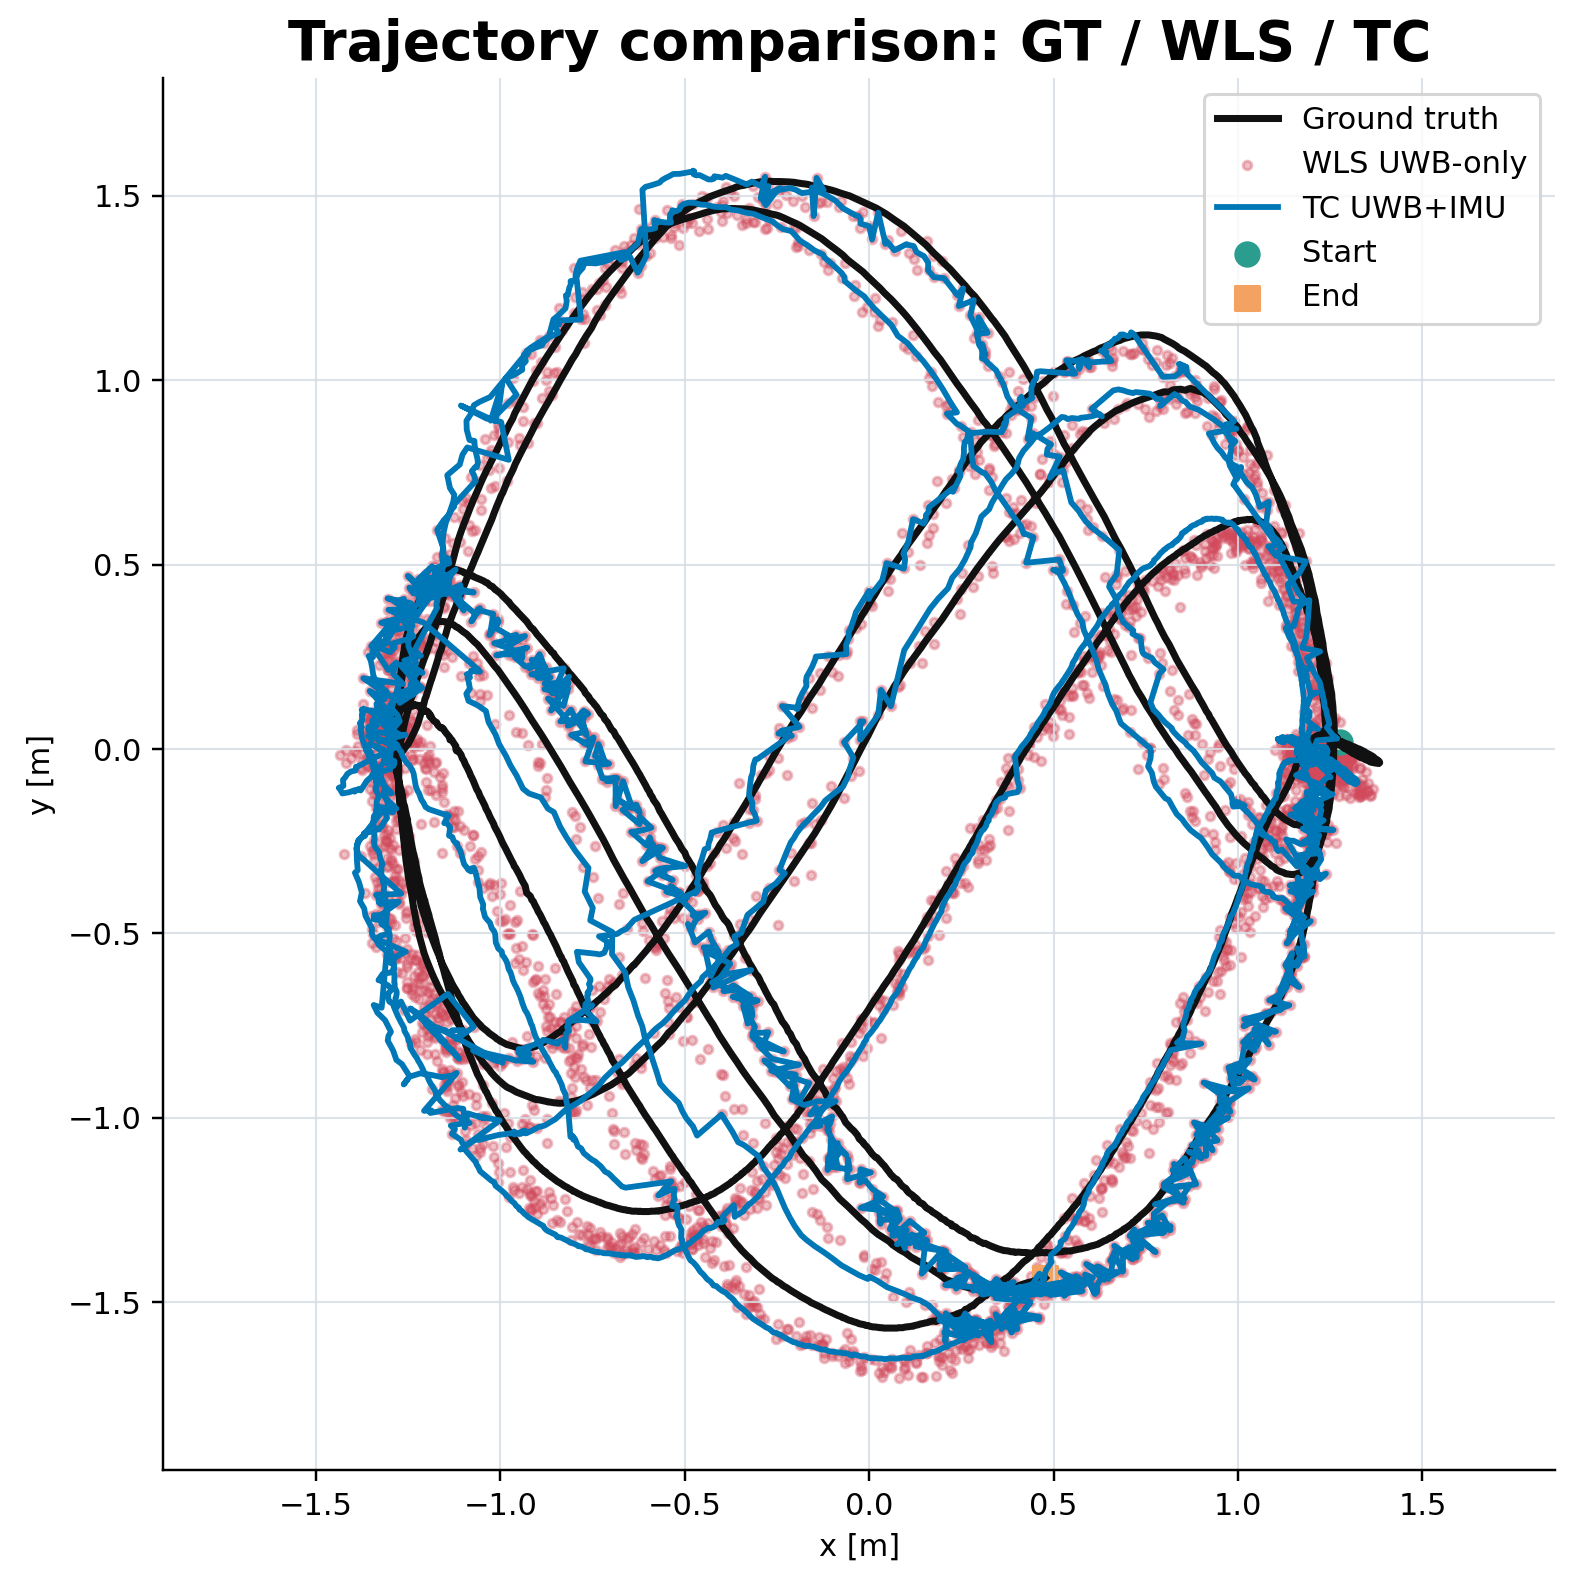
\includegraphics[width=0.82\linewidth]{trajectory_xy.png}
  \caption{Planar trajectory: ground truth, WLS, and TC.}
\end{figure}

\begin{figure}[H]
  \centering
  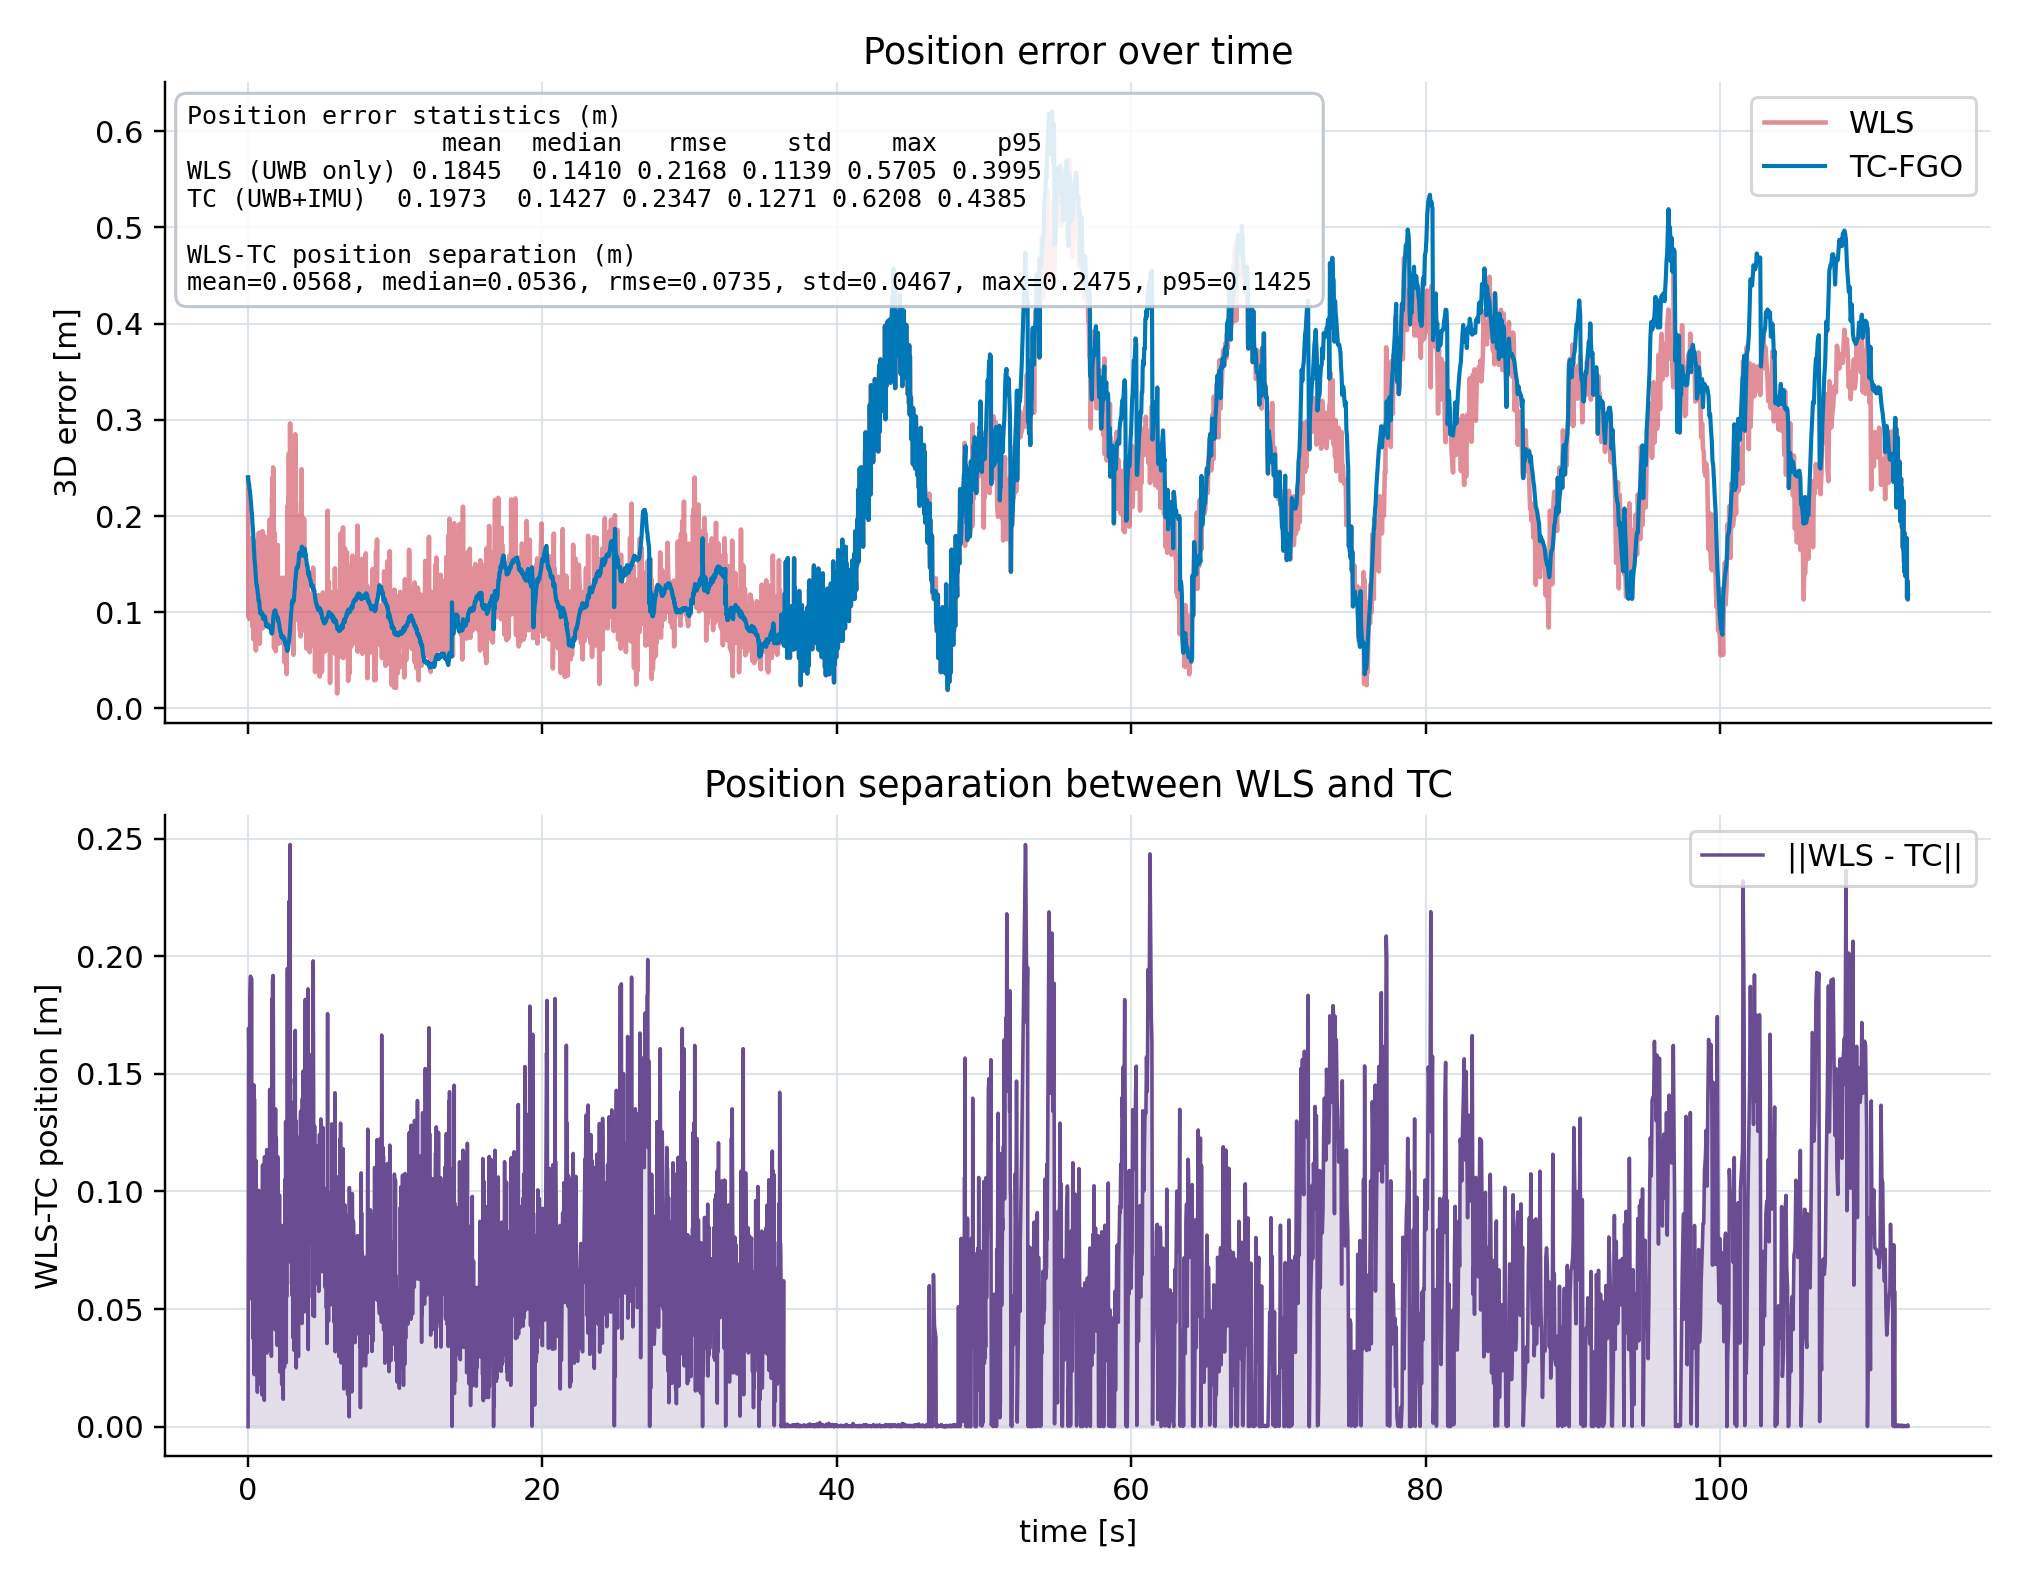
\includegraphics[width=0.9\linewidth]{error_timeseries.png}
  \caption{3D position error over time and TC-WLS error difference.}
\end{figure}

\begin{figure}[H]
  \centering
  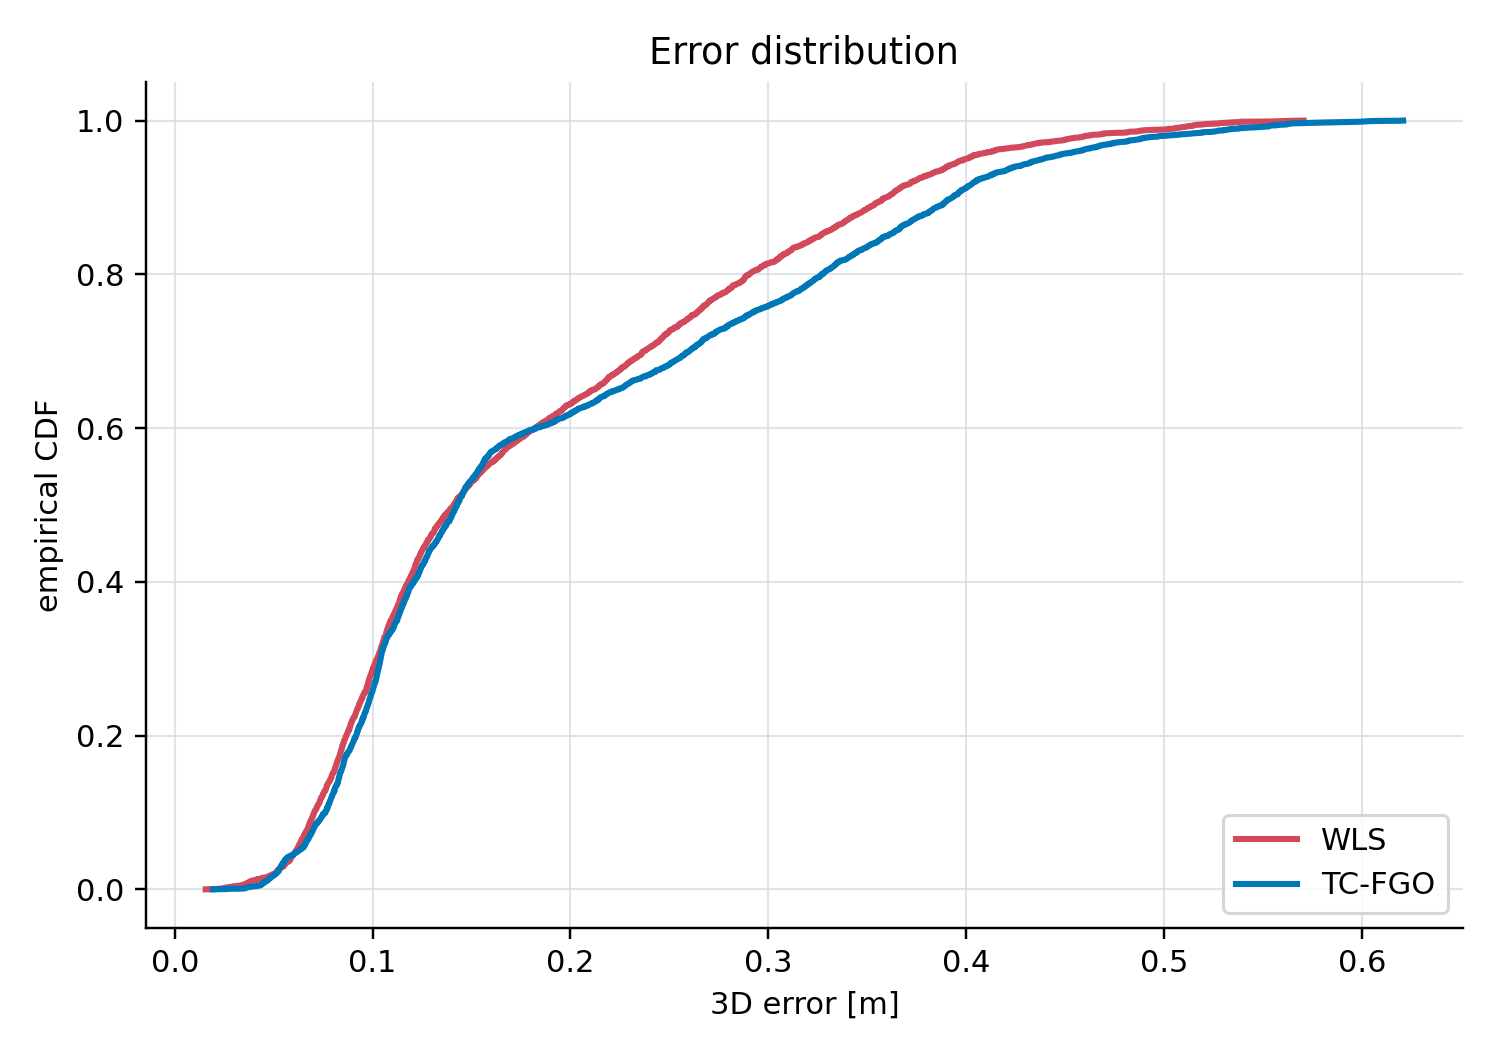
\includegraphics[width=0.72\linewidth]{error_cdf.png}
  \caption{Empirical cumulative distribution of 3D position error.}
\end{figure}

\begin{figure}[H]
  \centering
  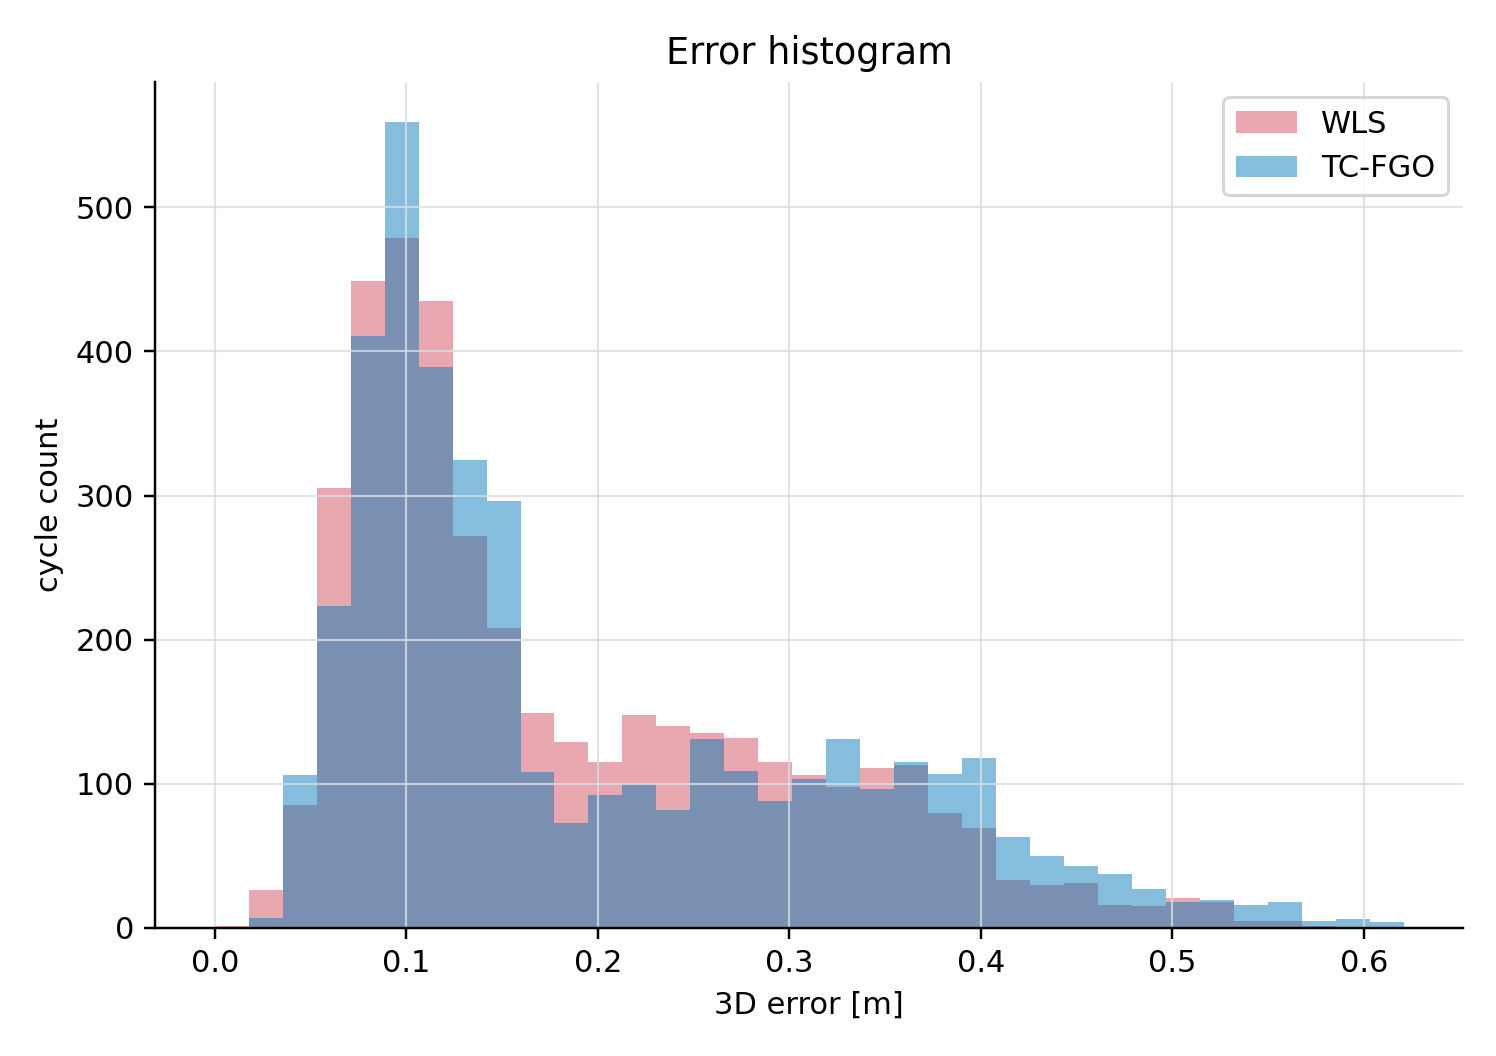
\includegraphics[width=0.72\linewidth]{error_histogram.png}
  \caption{Histogram of 3D position error.}
\end{figure}

\begin{figure}[H]
  \centering
  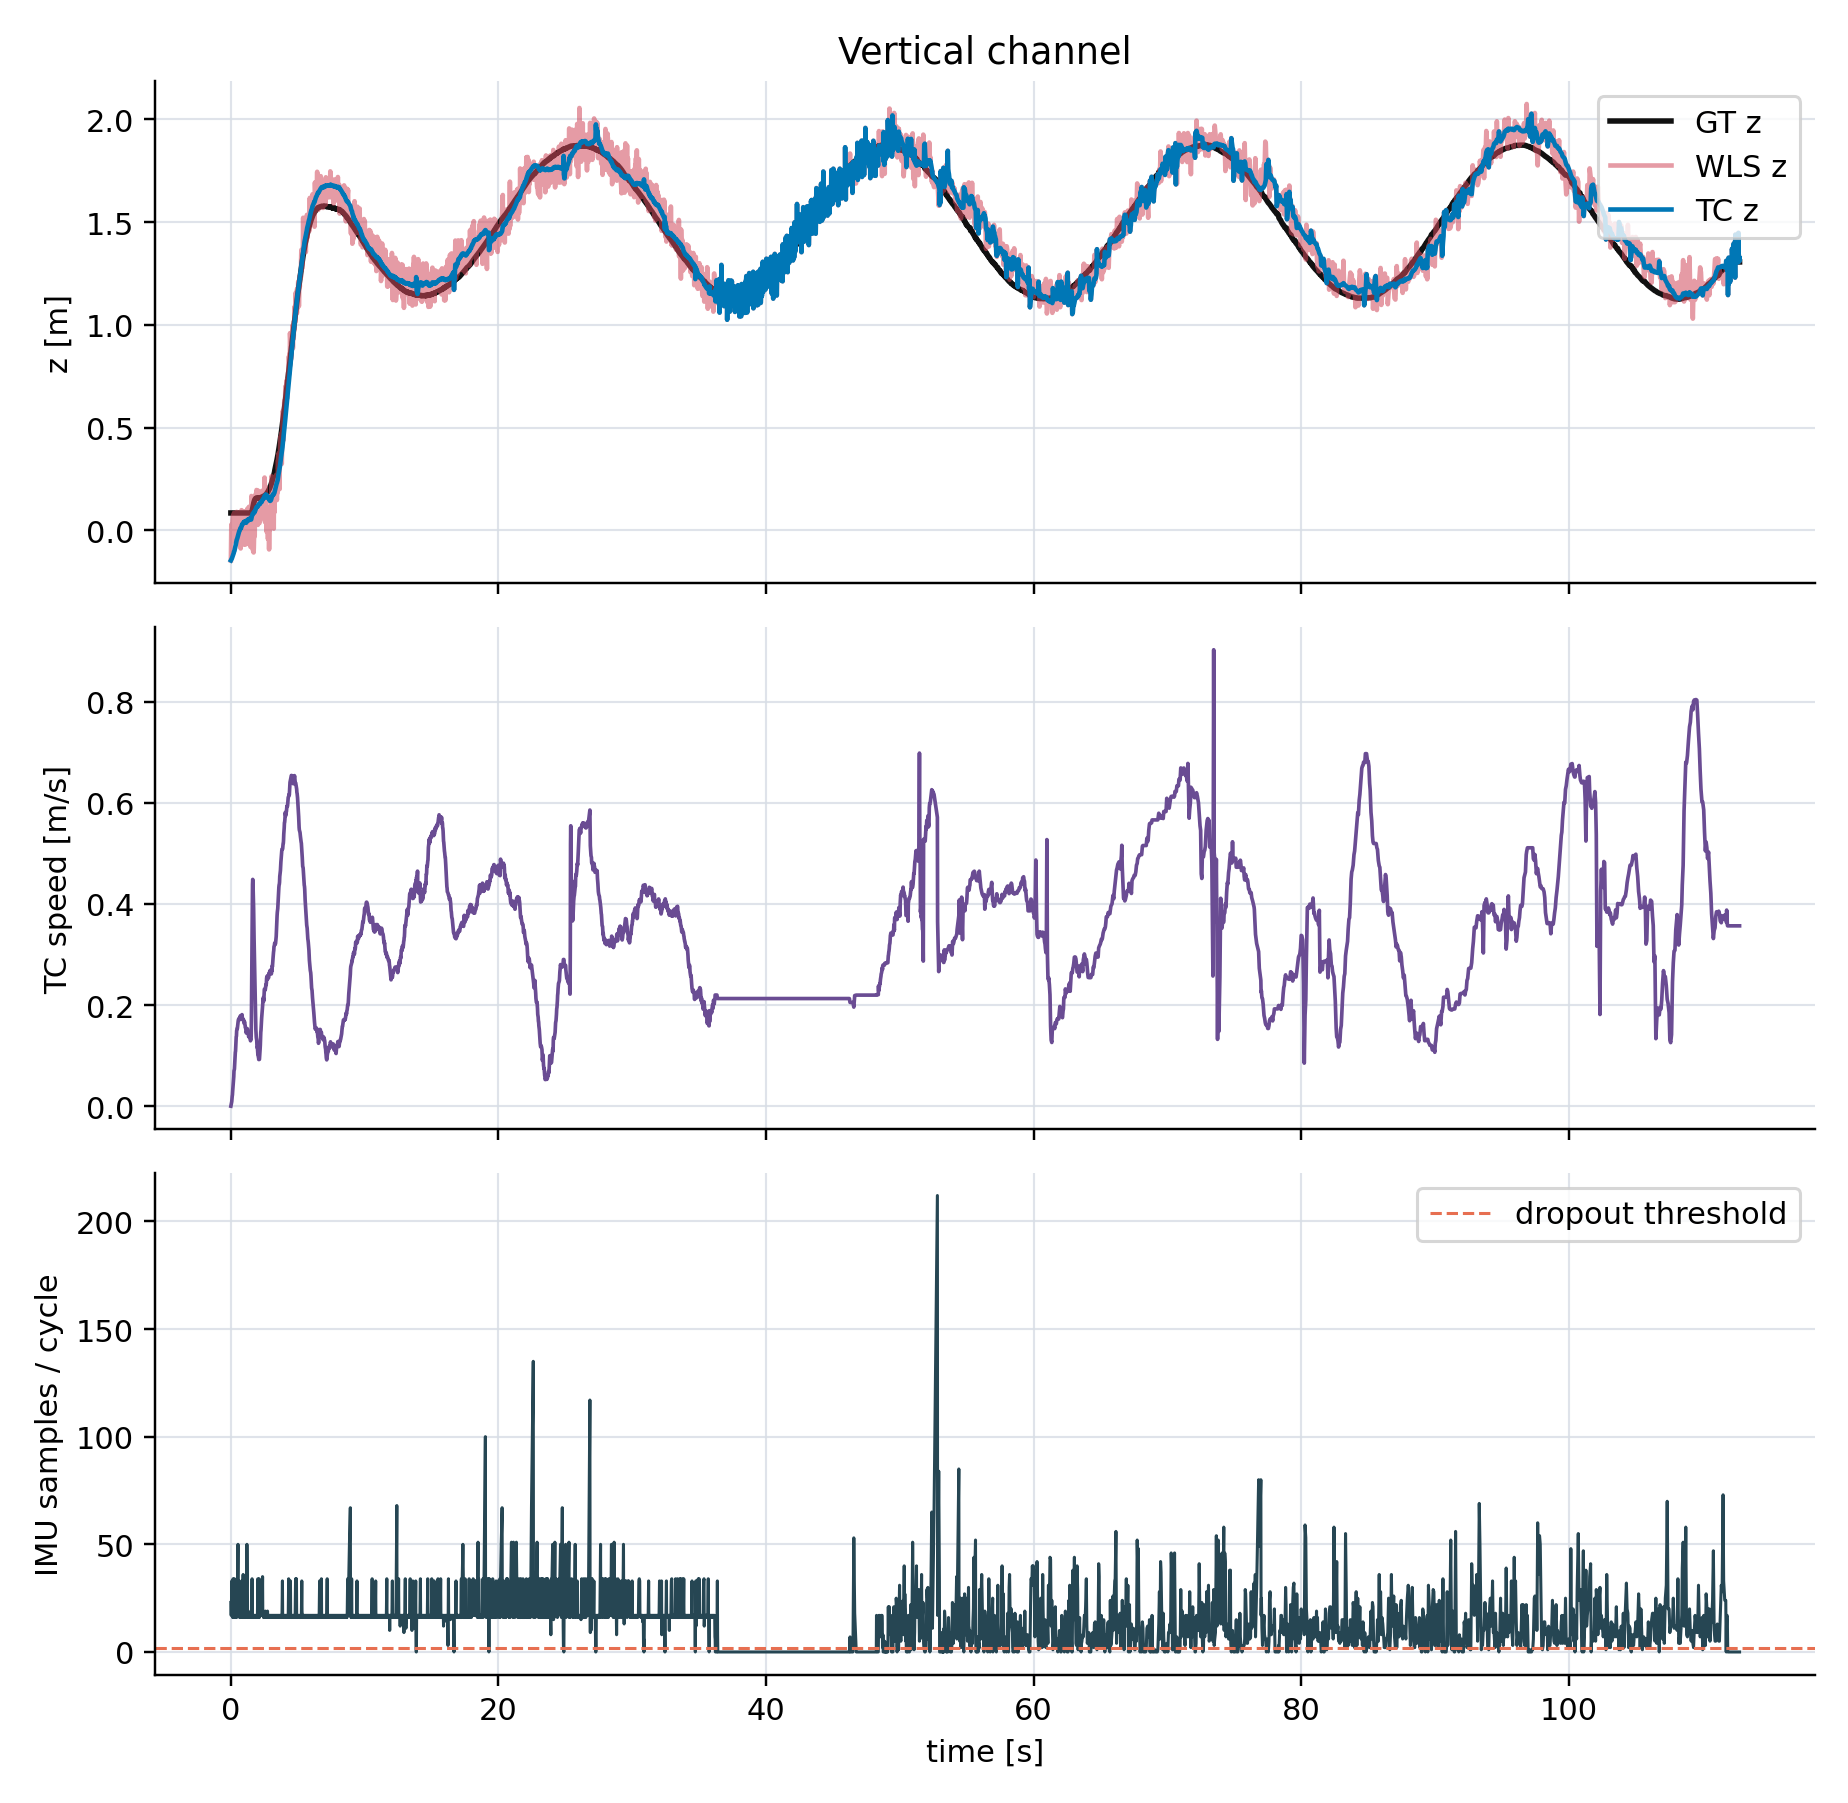
\includegraphics[width=0.9\linewidth]{state_diagnostics.png}
  \caption{Vertical state, TC speed, and IMU samples per UWB cycle.}
\end{figure}

\section{Interpretation}

The new constraints appear to solve the earlier catastrophic 12-second TC divergence: the early segment now has TC RMSE slightly lower than WLS. However, the full run shows TC accumulating more horizontal error than WLS in later segments. This suggests that the new strong constraints improve stability, but the graph is still not extracting a net horizontal accuracy gain from IMU information over long motion.

The most likely explanation is that WLS is already highly competitive for this anchor geometry, while the TC graph introduces extra dynamic assumptions: IMU preintegration, velocity regularization, attitude stabilization, and bias evolution. Those assumptions improve state continuity and altitude behavior, but they can also lag or bias the horizontal position when the direct UWB geometry is already good.

\section{Next Tuning Direction}

For this dataset, the best next tuning target is not more roll/pitch strength; the early-run divergence is already controlled. Instead:

\begin{itemize}[leftmargin=*]
  \item keep the attitude prior enabled;
  \item test a slightly weaker normal velocity prior, for example \(\sigma_v=0.7\) instead of \(0.5\);
  \item keep WLS rescue mode but consider activating it earlier in long-run sections, for example gate \SI{0.20}{m};
  \item add log columns for WLS rescue activation and roll/pitch to correlate late TC error with graph mode.
\end{itemize}

\section{Reproducibility}

Assets were generated with:
\begin{verbatim}
./report/generate_report_assets.py \
  --csv output/uwb_imu_trajectory_tc_260429.csv \
  --out-dir report/260429
\end{verbatim}

The animated replay is available as \texttt{trajectory\_replay.gif}.

\end{document}
